\title{Dokumentacja techniczna \\ programu ``Stacz kolejkowy''}
\author{
 Mateusz Klimek
}
\date{\vspace{-5ex}}
\documentclass[12pt]{article}

\usepackage{polski}
\usepackage[utf8]{inputenc}
\usepackage{url}
\usepackage{graphicx}
\usepackage{caption}

\begin{document}
\maketitle

\section{Budowanie}
Program można uruchomić na urządzeniach z Androidem 4.1 \textit{Jelly Bean}.
Aby zbudować projekt należy użyć polecenia \textit{`gradlew assembleDebug`} w terminalu w głównym katalogu z projektem. W razie kłopotów należy upewnić się czy na komputerze znajdują się wszystkie potrzebne pakiety z \textit{Android SDK}. Są one wypisane w pliku \textit{build.gradle}.

\section{Architektura}
\begin{figure}[h]
\centerline{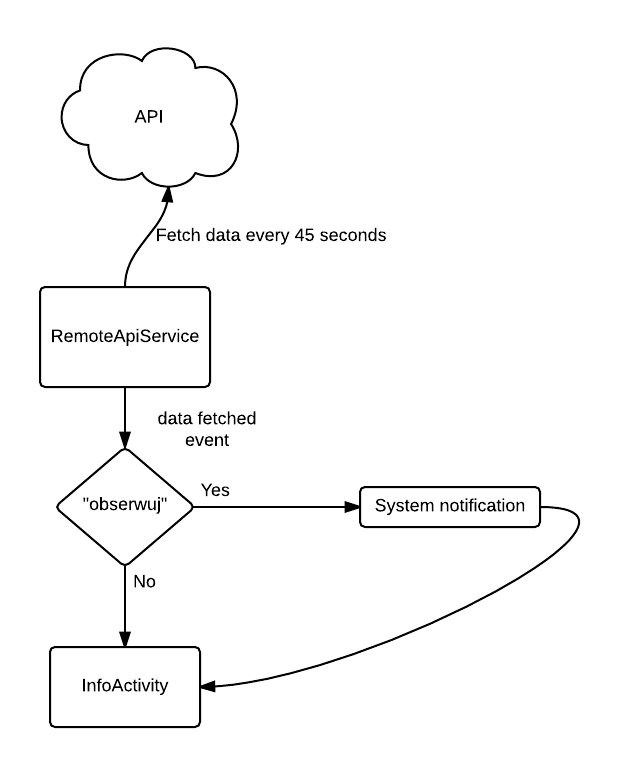
\includegraphics[width=0.43\textwidth]{arch}}
\caption{Uproszczona architektura systemu}
\label{fig:archas}
\end{figure}

W programie został zdefiniowany \textit{RemoteApiService}, czyli serwis działający w tle, nawet gdy aplikacja nie jest widoczna dla użytkownika. Zadaniem serwisu jest cykliczne wysyłanie żądań do serwera i informowanie o tym wszystkich zainteresowanych poprzez wyemitowanie odpowiedniego zdarzenia. 

\textit{InfoActivity} reprezenuje okno programu w którym użytkownik widzi informacje na temat kolejki. Jest ono klientem serwisu \textit{RemoteApiService}, więc może odbierać zdarzenia o zaaktualizowaniu danych i zaprezenować użytkownikowi odpowiednie dane. W tym oknie jest również możliwość włączenia opcji ``Obserwuj'', która powoduje, że nawet po wyjściu z aplikacji użytkownik będzie mógł otrzymywać powiadomienia o zmiane w kolejce poprzez notyfikacje systemowe. Po tapnięciu w taką notyfikację system przeniesie użytkownika do aplikacji.
\section{Biblioteki}
\begin{itemize}
 \item Dagger\footnote{\url{https://github.com/square/dagger}} - implementacja wzorca \textit{Dependency Injection}.
 \item Retrofit\footnote{\url{https://github.com/square/retrofit}} - konsumowanie serwisu typu \textit{REST}.
 \item Otto\footnote{\url{https://github.com/square/otto}} - implementacja wzorca \textit{Publish-Subscribe}.
 \item OkHttp\footnote{\url{https://github.com/square/okhttp}} - klient HTTP z możliwością konfigurowania certyfikatów.
 \item Calligraphy\footnote{\url{https://github.com/chrisjenx/Calligraphy}} - ładowanie dowolnych czcionek.
\end{itemize}

\section{Inne}
W razie pytań zapraszam na mateusz.kliemk.art@gmail.com :)

\end{document}